\documentclass[british,10pt]{beamer}
\usepackage{pifont}

% Beamer specific settings

% Other styles can be used instead of Boadilla, e.g., to add an index column.
\mode<presentation>
{
  \usetheme{Boadilla} % Without index, with footer
}

\title{Building a better VHDL testing environment}
\author[J. Guillaume]{Joren Guillaume}
\date[DEC'14, Gent]{Prelimenary Presentation}
\institute[Ghent University]
{
  FEA\\
  Ghent University
}

% This command makes the logo appear at the right side which does not fit
% the UGent style. A solution is found further below.
% \logo{\includegraphics[scale=0.25]{logolabel.jpg}}

\AtBeginSubsection[]
{
  \begin{frame}<beamer>\frametitle{Outline}
    \tableofcontents[currentsection,currentsubsection]
  \end{frame}
}

\setbeamersize{text margin left=1cm}
\setbeamersize{text margin right=1cm}

\begin{document}


% Titlepage containing the logo of the Faculty (Engineering in this example)
\begin{frame}[plain]
\mode<presentation>{
\includegraphics[width=\textwidth]{tw.pdf}}
  \titlepage
\end{frame}


% UGent logo at left side from second slide on.
\setbeamertemplate{sidebar left}{ 
\vfill 
\rlap{%\hskip0.1cm 
 
\includegraphics[scale=0.3]{logolabel2.jpg} } 
\vskip20pt 
}

\begin{frame}<beamer>\frametitle{Outline}
  \tableofcontents
\end{frame}

\section{Introduction}
\subsection{VHDL}

\begin{frame}\frametitle{VHDL}
VHDL
\begin{itemize}
\item VHSIC Hardware Description Language
\item Used for describing digital and mixed-signal systems 
\item Developed by U.S. Department of Defense
\begin{itemize}
\item Document \ding{222} Simulate \ding{222} Synthesize
\end{itemize}
\end{itemize}
\end{frame}

\begin{frame}\frametitle{VHDL - design flow}
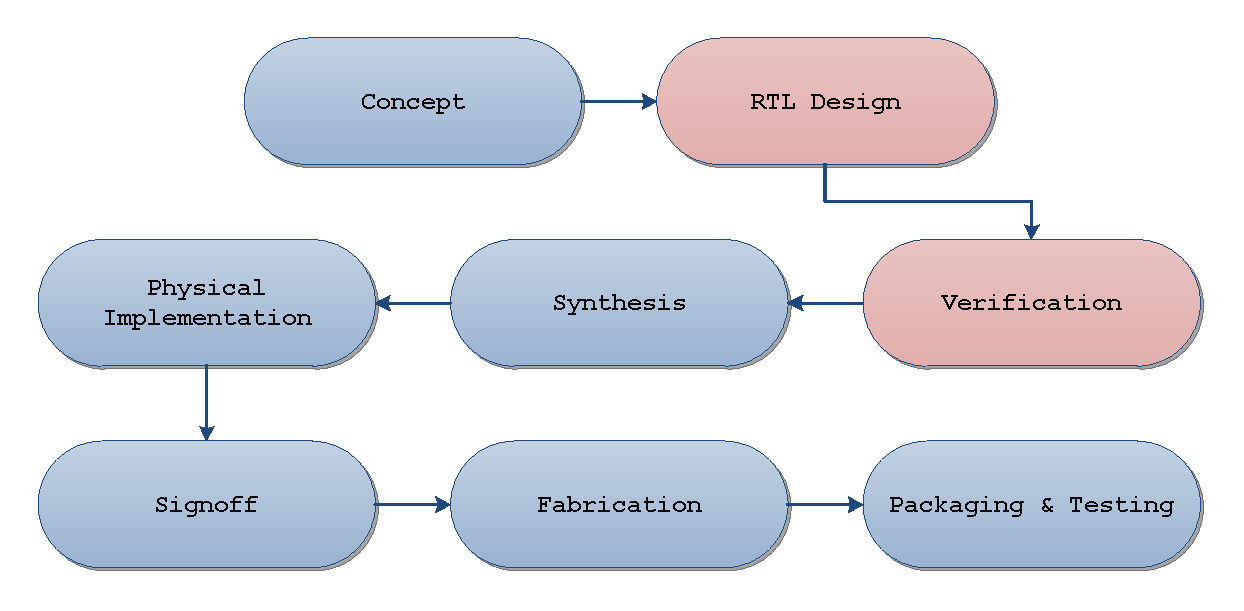
\includegraphics[width=\textwidth]{images/VHDLflow.pdf}
\end{frame}

\subsection{Testing VHDL}

\begin{frame}\frametitle{Testing VHDL}
Testbenches
\begin{itemize}
\item Unit Under Test (UUT)
\item Signal drivers, stimuli \& processes
\item Assertions and output tracking
\begin{itemize}
\item Comparison to "golden reference"
\item Manual check
\item Wave-check
\end{itemize}
\end{itemize}
\vspace{0.25cm}
Problems
\begin{itemize}
\item Non-standardized process
\item Single point of failure
\end{itemize}
\end{frame}

\begin{frame}\frametitle{Modelsim - waves}
\centering
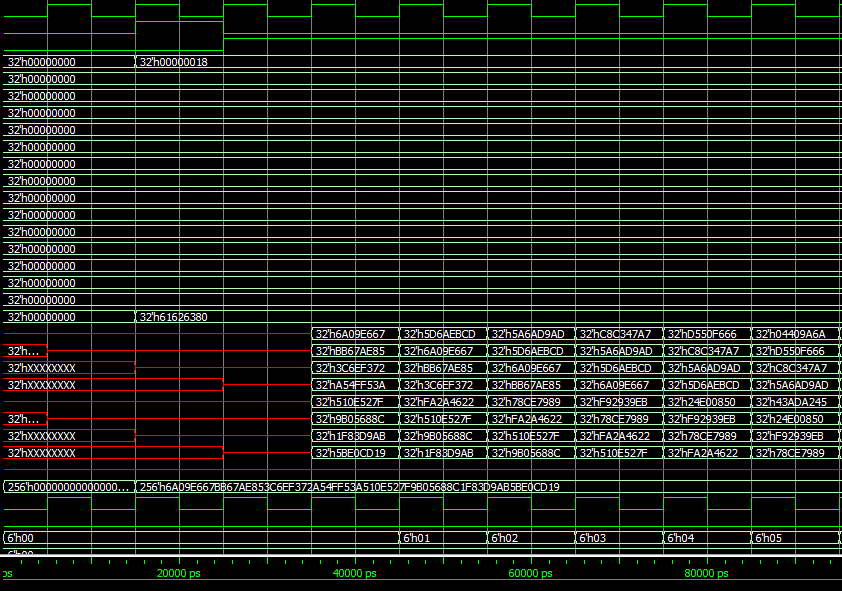
\includegraphics[width=0.9\textwidth]{images/waves.png}
\end{frame}

\section{Proposed solution}

\subsection{VHDL testing Framework}

\begin{frame}\frametitle{VHDL testing framework}
Standardized testing framework
\begin{itemize}
\item Based on Test Driven Development (TDD)
\item Cross platform
\item Utility library
\begin{itemize}
\item Standardized testbenches
\item Swift coding
\end{itemize}
\item Script-based processing \ding{222} Standardized processing \& output
\item Continuous Integration (CI) system
\end{itemize}
\end{frame}

\subsection{Test Driven Development}

\begin{frame}\frametitle{Test Driven Development}
\begin{columns}
\begin{column}{0.6\textwidth}
Test Driven Development
\begin{itemize}
\item Software development technique
\item Proven to significantly reduce errors
\item All behaviour is tested
\item Unit testing \& short development cycle
\item Red - Green - Refactor
\end{itemize}
\end{column}
\column{0.4\textwidth}
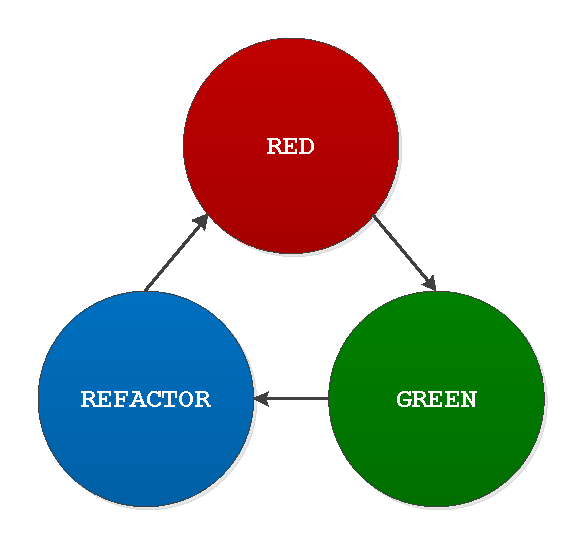
\includegraphics[width=\textwidth]{images/tdd.pdf}
\end{columns}
\end{frame}

%\begin{frame}\frametitle{TDD - design flow}
%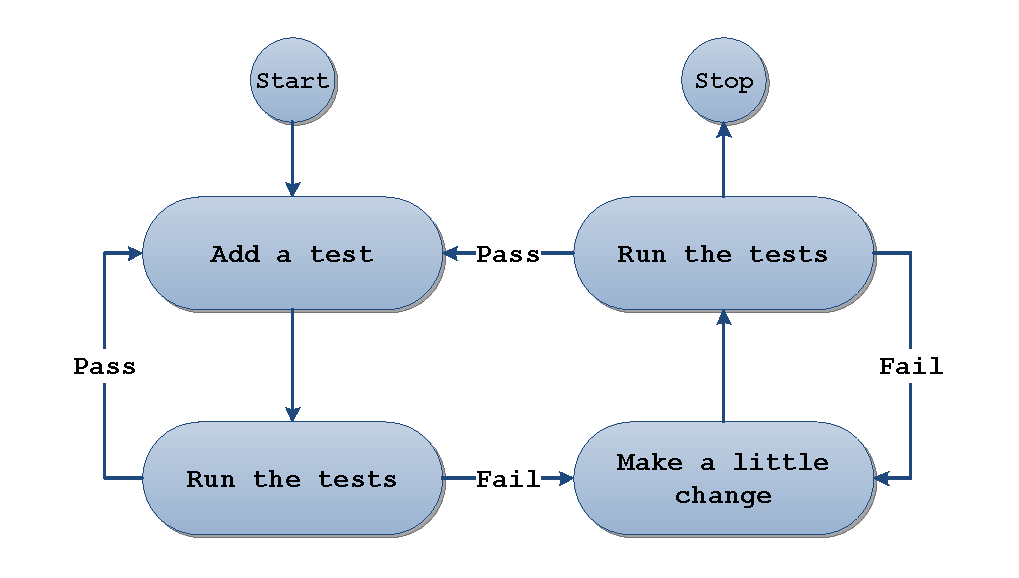
\includegraphics[width=\textwidth]{images/TDDflow2.pdf}
%\end{frame}

\subsection{Utility library}

\begin{frame}\frametitle{Specialized library}
\begin{columns}
\begin{column}{0.6\textwidth}
Bitvis utility library
\begin{itemize}
\item Expands VHDL functions
\begin{itemize}
\item Easy value checking
\item Clock \& pulse generators
\item String handling \& random generation
\item Easy output logging
\end{itemize}
\item Quick \& uniform coding
\item Compatible with all VHDL versions
\end{itemize}
\end{column}
\column{0.5\textwidth}

\includegraphics[width=0.6\textwidth]{images/bitvis.png}
\end{columns}
\end{frame}

\subsection{Script-based processing}

\begin{frame}\frametitle{Script-based processing}
Specialized python script
\vspace{1cm}
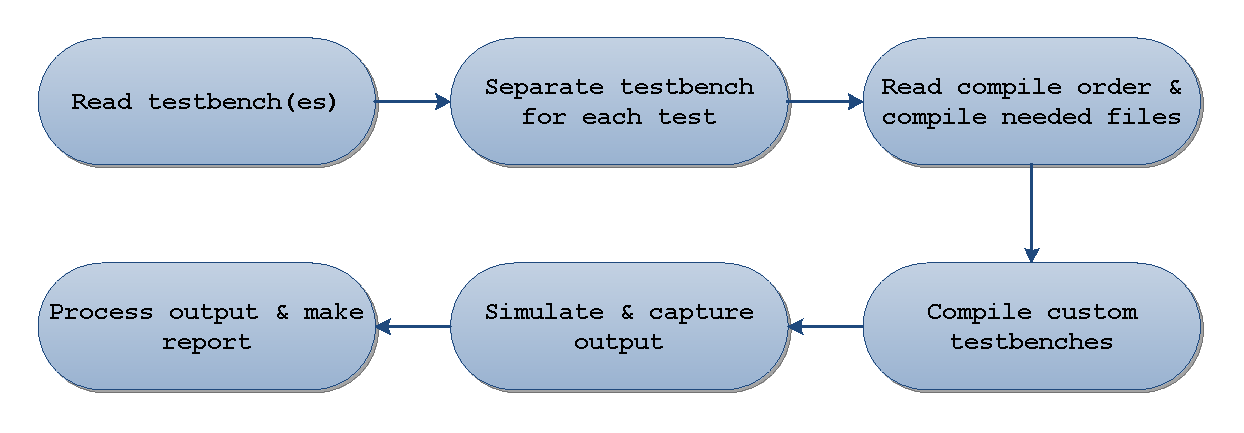
\includegraphics[width=\textwidth]{images/Scriptflow.pdf}
\end{frame}

\begin{frame}\frametitle{Script-based processing}
Features
\begin{itemize}
\item Standalone functions
\item Customizable process
\item Text \& JUnit format reports
\item Automated file cleanup
\end{itemize}
\end{frame}

\subsection{Continuous Integration}

\begin{frame}\frametitle{Continuous Integration}
\begin{columns}
\begin{column}{0.6\textwidth}
Hudson-CI
\begin{itemize}
\item Centralized, automated testing
\item Revision control integration (e.g. Git)
\item Statistics on success
\item Standardized test reports (JUnit)
\item Very customizable
\end{itemize}
\end{column}
\column{0.5\textwidth}

\includegraphics[width=0.6\textwidth]{images/hudson.png}
\end{columns}
\end{frame}

\begin{frame}\frametitle{Hudson interface}
\centering
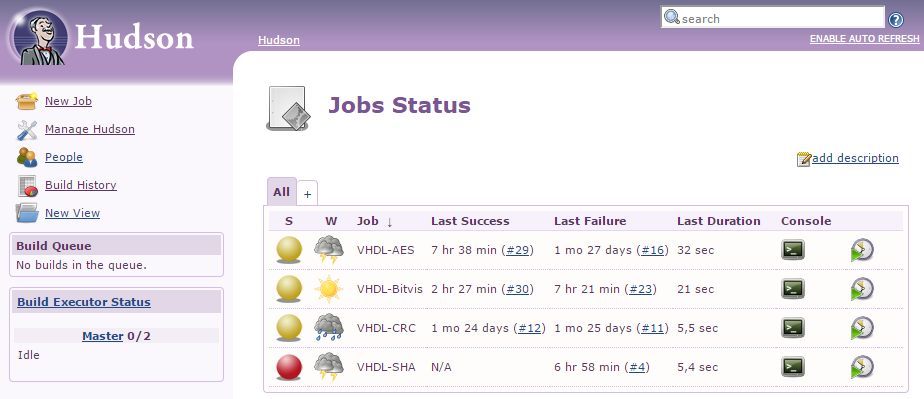
\includegraphics[width=\textwidth]{images/hudsoninterface.png}
\end{frame}

\begin{frame}\frametitle{Hudson statistics}
\centering
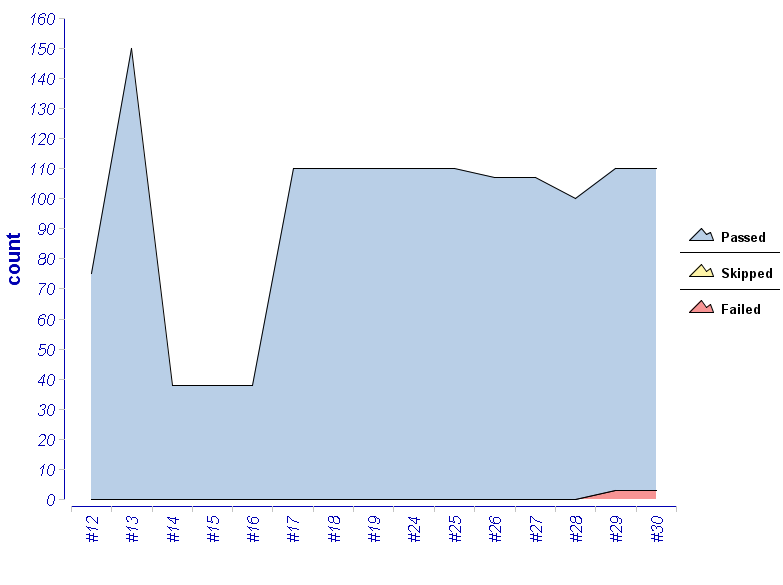
\includegraphics[width=0.8\textwidth]{images/hudsonstats.png}
\end{frame}

\begin{frame}\frametitle{Framework design flow}
\centering
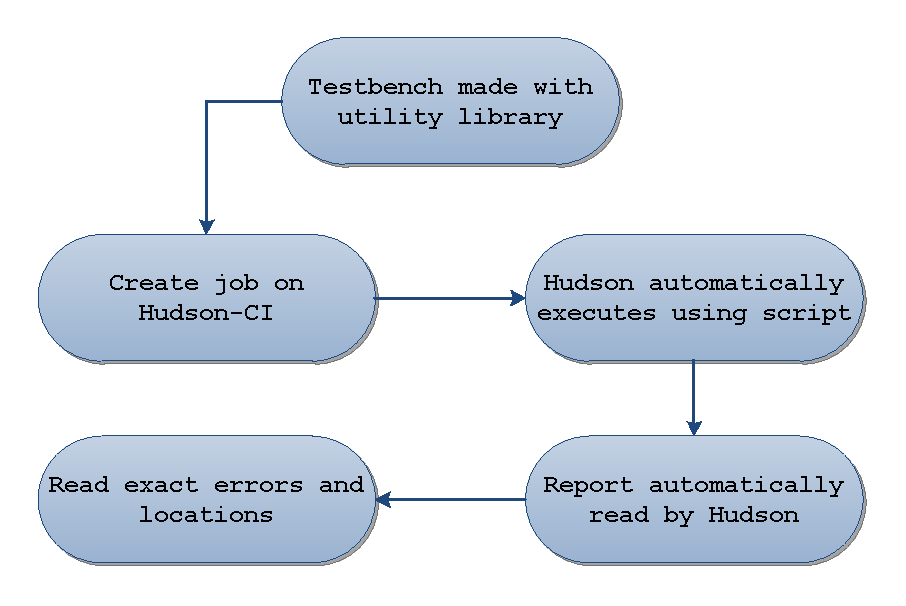
\includegraphics[width=0.8\textwidth]{images/Frameworkflow.pdf}
\end{frame}

\section{Concluding}

\subsection{Problems}
\begin{frame}\frametitle{Problems}
\begin{itemize}
\item VHDL has no reflection
\begin{itemize}
\item Circumvent with higher level language
\end{itemize}
\item Code duplication increases compile \& simulation time
\begin{itemize}
\item Implement regression testing
\item Smart code filtering
\end{itemize}
\item Simulation is not synthesis
\begin{itemize}
\item Wait statements, wrong sensitivity list ...
\end{itemize}
\end{itemize}
\end{frame}

\subsection{Future work}

\begin{frame}\frametitle{Future work}
\begin{itemize}
\item Improving base script
\begin{itemize}
\item Better integration utility library
\item More options
\end{itemize}
\item Smart code analysis
\item Regression testing
\item Proper documentation \& examples
\end{itemize}
\end{frame}

\subsection{Demo}

\begin{frame}\frametitle{Demo}
\centering
\Huge Demo
\end{frame}

\end{document}
